\documentclass[11pt,letterpaper]{article}
\usepackage[margin=0.8in]{geometry}
\usepackage{amsmath,amssymb,booktabs,array,graphicx,microtype,enumitem,xcolor}
\usepackage[colorlinks=true,urlcolor=blue!45!black,linkcolor=black]{hyperref}
\usepackage{titlesec}
\titleformat{\section}{\large\bfseries}{\thesection}{0.6em}{}
\titlespacing*{\section}{0pt}{10pt}{6pt}
\setlength{\parindent}{0pt}\setlength{\parskip}{6pt}
\setlist{nosep,leftmargin=1.5em}\pagestyle{plain}
\begin{document}
\begin{center}
{\Large\bfseries FINCB9339 Systematic Investment Strategies}\\[5pt]
{\large Homework 5: Dual Momentum}\\[5pt]
Hanyu Zhang (hz3069)
\end{center}
\section*{Summary of answers}
The four-module dual momentum portfolio earned a 6.08340\% annualized geometric return, a 0.58737 excess-return Sharpe ratio and a \(-14.05541\%\) maximum month-end drawdown over June 2008--June 2026. Its strongest result is downside reduction, rather than a general improvement in return.

\textbf{(a) Data and portfolio.} Nine USD-denominated ETFs implement the paper's four modules: equities (VTI/EFA), credit (HYG/LQD), real estate (VNQ/REM), and economic stress (GLD/TLT). Each module receives 25\% of capital and can move entirely into the same short-Treasury cash proxy, SHV. Daily dividend- and split-adjusted prices are sampled at month-end. Common levels start in May 2007, with 217 monthly holding returns from June 2008 through June 30, 2026. The sample overlaps the paper and captures the severe phase of the financial crisis. ETF inception prevents a full 2000--2009 comparison.

\textbf{(b) Implementation.} At month-end, select the better-performing risky asset over the latest 12 months, including the most recent month. Hold it during the subsequent month only if its trailing return exceeds SHV's; otherwise hold SHV. Rebalance the four sleeves to equal weights monthly. The accompanying project contains frozen source data, all monthly signals and holdings, asset and strategy returns, formulas, and an offline reproduction procedure. Factor-model alpha comparisons are omitted as permitted.

\textbf{(c) Findings.} Dual momentum's full-sample Sharpe exceeds the static portfolio's 0.48750, but its CAGR falls below the static portfolio's 6.52178\%. In 2012--June 2026, the respective Sharpe ratios are 0.51158 and 0.54822. These results provide only partial support for Antonacci's broad performance claims.

\textbf{(d) Extra credit.} A fixed 2-percentage-point relative-momentum switching buffer raises full-sample CAGR to 6.33698\% and Sharpe to 0.61771, while reducing turnover. Its extension-sample Sharpe improvement has a confidence interval containing zero. It is a promising implementation refinement, not an established superior strategy.

\textbf{Interpretation.} A relative winner can still have an unfavorable trend. Cash substitution limits persistent losses, but reacts slowly to sudden shocks and can miss rapid recoveries. Gold and long Treasuries add diversification, but neither is a guaranteed safe asset. Results are an ETF adaptation of the paper, rather than an exact index replication.

\newpage
\section{Data and economic mapping: question (a)}
Antonacci (2013, January 28 version) combines relative strength and a Treasury-bill hurdle within four economically distinct modules:
\begin{center}\small
\begin{tabular}{l>{\raggedright\arraybackslash}p{3.8cm}>{\raggedright\arraybackslash}p{7cm}}\toprule
Module & ETF alternatives & Economic interpretation and departures\\\midrule
Equities & VTI: US total stock market; EFA: MSCI EAFE &
Domestic versus developed foreign equities. EFA excludes emerging markets, unlike the paper's post-1987 EAFE+ composite. VTI includes small stocks.\\
Credit & HYG: high-yield corporates; LQD: investment-grade corporates &
Default-risk contrast. LQD spans maturities and differs in duration from the paper's intermediate credit index.\\
Real estate & VNQ: US real estate; REM: mortgage REITs &
Property ownership versus mortgage financing. VNQ is broader than an exact equity-REIT index. Mortgage REITs contain leverage, spread and funding risk.\\
Stress & GLD: physical gold trust; TLT: 20+ year Treasuries &
Uncertainty and nominal-duration exposures. ETF expenses and market pricing differ from physical gold and index returns.\\
Common cash & SHV: 0--1 year US Treasuries &
Common hurdle and fallback. Low-duration government debt, not a constant-value account or the paper's 3-month bill index.\\\bottomrule
\end{tabular}
\end{center}
\textbf{Source and dates.} Prices come from Yahoo Finance's daily chart endpoint, one frozen JSON response per ticker. Its adjusted-close field incorporates splits and distributions. All series are USD market prices, including EFA's embedded currency exposure. No separate dividend yield, funding return, or expense ratio is added or subtracted. Fund expenses are embedded in observed returns. Retrieval timestamps, full request URLs and SHA-256 hashes accompany the data.
\begin{center}\small\begin{tabular}{lrrr}\toprule
Asset & First daily quote & Last quote & Daily rows\\\midrule
VTI & 2006-01-03 & 2026-06-30 & 5154\\
EFA & 2006-01-03 & 2026-06-30 & 5154\\
HYG & 2007-04-11 & 2026-06-30 & 4836\\
LQD & 2006-01-03 & 2026-06-30 & 5154\\
VNQ & 2006-01-03 & 2026-06-30 & 5154\\
REM & 2007-05-04 & 2026-06-30 & 4819\\
GLD & 2006-01-03 & 2026-06-30 & 5154\\
TLT & 2006-01-03 & 2026-06-30 & 5154\\
SHV & 2007-01-11 & 2026-06-30 & 4897\\
\bottomrule\end{tabular}\end{center}
The request covers January 2006--June 2026. REM's first available quote, May 4, 2007, determines the common start. The last actual US trading session of each calendar month supplies the monthly level. All nine assets share these sessions after their first quote. There are no missing values after inception, duplicate dates, imputations, winsorization, or synthetic pre-inception histories. Leading unavailable observations are excluded. A 12-month signal needs 13 levels; May 2008 is the first decision date and June 2008 the first holding month.

\newpage
\section{Portfolio rules and return measurement: question (b)}
Let \(P_{i,t}\) be the adjusted close on the last trading session of month \(t\). Arithmetic total returns and 12-month momentum are
\[
r_{i,t}=\frac{P_{i,t}}{P_{i,t-1}}-1,\qquad
M_{i,t}=\frac{P_{i,t}}{P_{i,t-12}}-1
       =\prod_{j=0}^{11}(1+r_{i,t-j})-1.
\]
The current month enters the signal; no last-month reversal adjustment is used. Within module \(m\), whose risky alternatives are \(\mathcal A_m\), select
\[
i^*_{m,t}=\arg\max_{i\in\mathcal A_m}M_{i,t},\qquad
h_{m,t}=
\begin{cases}
i^*_{m,t},&M_{i^*_{m,t},t}>M_{\mathrm{SHV},t},\\
\mathrm{SHV},&\text{otherwise}.
\end{cases}
\]
Exact risky-asset ties follow the listed ticker order. Equality to cash selects cash. Equal-weight the four modules, not all nine assets:
\[
w_{i,t}=\frac14\sum_{m=1}^{4}\mathbf1\{h_{m,t}=i\},\qquad
R_{t+1}=\sum_i w_{i,t}r_{i,t+1}.
\]
Weights are nonnegative and sum to one. Multiple sleeves selecting SHV aggregate into one cash holding. Each sleeve holds its selection throughout the month; the composite resets to 25\% per sleeve monthly. These are funded returns, unlike the self-financing FX excess returns in earlier homework.

\textbf{Timing.} A score observed at the end of \(t\) never earns the already-completed return \(r_{i,t}\). The monthly backtest uses the conventional frictionless month-end decision/execution boundary. Exact closing prices cannot be both fully observed and traded instantaneously in practice. An additional full-month signal delay is reported separately. A precise next-session implementation requires intraday or next-open total-return accounting.

\textbf{Performance definitions.} With \(N\) months and \(W_0=1\),
\[
 W_n=\prod_{t=1}^{n}(1+R_t),\quad
 \bar R_{\rm ann}=12\bar R,\quad
 {\rm CAGR}=W_N^{12/N}-1,\quad
 \sigma_{\rm ann}=\sqrt{12}\,s(R).
\]
The Sharpe ratio uses realized monthly cash excess returns:
\[
 {\rm SR}=\sqrt{12}\frac{\overline{R-r_{\mathrm{SHV}}}}
 {s(R-r_{\mathrm{SHV}})},\qquad
 {\rm MDD}=\min_n\left(\frac{W_n}{\max(1,W_1,\ldots,W_n)}-1\right).
\]
Standard deviations use \(N-1\); skewness and excess kurtosis use bias-adjusted sample estimators. The 5\% quantile uses linear interpolation; expected shortfall averages observed returns at or below that quantile. Negative tail statistics and MDD denote losses. Drawdown includes initial capital and is measured at month-ends; intramonth losses can be larger.

\newpage
\section{Composite performance and distributions: question (c)}
All main comparisons use June 2008--June 2026. Static resets to one eighth in each risky asset monthly. Relative selects each module's risky winner without the cash hurdle. Absolute allocates half a sleeve to each risky asset when it beats cash, otherwise placing that half in SHV. Buffer is defined in Section 7.
\begin{center}\small\begin{tabular}{lrrrr}\toprule
Portfolio & CAGR (\%) & Vol. (\%) & Sharpe & MDD (\%)\\\midrule
Dual & 6.08340 & 8.38713 & 0.58737 & -14.05541\\
Relative & 7.22606 & 11.55408 & 0.54834 & -35.50730\\
Absolute & 4.43381 & 6.63083 & 0.48425 & -14.84271\\
Static & 6.52178 & 11.62646 & 0.48750 & -30.65167\\
Buffer & 6.33698 & 8.36081 & 0.61771 & -14.25792\\
US equities & 11.64644 & 16.25196 & 0.67893 & -46.56268\\
Exposure control & 5.54493 & 9.20467 & 0.48750 & -24.58785\\
\bottomrule\end{tabular}\end{center}
\begin{center}\small\begin{tabular}{lrrrrr}\toprule
Portfolio & Arith. (\%) & Worst (\%) & ES$_{5\%}$ (\%) & Skew & Ex. kurt.\\\midrule
Dual & 6.27126 & -8.69443 & -5.10388 & -0.44740 & 1.47651\\
Relative & 7.67483 & -16.82138 & -8.09320 & -1.03809 & 3.63526\\
Absolute & 4.56863 & -12.05125 & -4.33575 & -1.46569 & 7.54520\\
Static & 7.01718 & -14.38471 & -7.83871 & -0.77873 & 3.26225\\
Buffer & 6.50884 & -8.69443 & -5.06120 & -0.43106 & 1.48751\\
\bottomrule\end{tabular}\end{center}
The combined rule improves Sharpe relative to the static and relative portfolios, but sacrifices compounded return. Relative momentum earns more than dual momentum, at the cost of a much larger drawdown. Absolute momentum alone produces a lower CAGR and Sharpe than dual momentum, suggesting that relative selection contributes in this universe. These comparisons isolate the mechanisms within the same data.

For dual momentum, one dollar grows to \$2.90932 before investor-level costs and taxes. The worst month and expected shortfall remain materially negative. Absolute momentum is a trend rule, not a contractual floor. A favorable trailing trend does not exclude a sharp loss next month. Appendix D displays both tails.

\textbf{Is protection simply less risky exposure?} Average risky allocation is 79.14747\%. The Exposure control holds this fixed fraction in the static basket and the remainder in SHV, rebalanced monthly. Its MDD is -24.58785\%, versus dual momentum's \(-14.05541\%\). Lower average exposure explains part, but not all, of the drawdown difference. This control uses a full-sample average and is descriptive, not an implementable ex-ante strategy. Its Sharpe equals Static's because its excess returns are a positive constant multiple of Static's excess returns.

US equities deliver higher return and Sharpe over this sample. That is an important opportunity cost of diversified defensive allocation. It contradicts any expectation that the strategy uniformly preserves equity upside while lowering risk.

\newpage
\section{The four modules}
\begin{center}\small\begin{tabular}{lrrrr}\toprule
Portfolio & CAGR (\%) & Vol. (\%) & Sharpe & MDD (\%)\\\midrule
Equities & 8.05356 & 12.66591 & 0.56994 & -21.99587\\
Credit & 5.11303 & 5.54046 & 0.68513 & -8.75316\\
REITs & 3.31203 & 14.42170 & 0.20466 & -40.06499\\
Stress & 5.91262 & 16.09515 & 0.35608 & -25.28571\\
\bottomrule\end{tabular}\end{center}
Credit has the highest module Sharpe. Real estate has the weakest Sharpe and a substantial drawdown despite its cash option. Mortgage REITs combine rate, credit, leverage and funding exposure. A positive trailing return can disappear rapidly when liquidity changes. Gold and nominal long-duration debt have different sensitivities, helping explain the stress sleeve's mixed performance.
\begin{center}\small\begin{tabular}{lrrrr}\toprule
Module & Rule & CAGR (\%) & Sharpe & MDD (\%)\\\midrule
Credit & dual & 5.11303 & 0.68513 & -8.75316\\
Credit & relative & 5.48372 & 0.53461 & -15.24930\\
Credit & static & 4.76483 & 0.42659 & -20.17304\\
Equities & dual & 8.05356 & 0.56994 & -21.99587\\
Equities & relative & 9.64819 & 0.56736 & -48.38930\\
Equities & static & 8.31289 & 0.48919 & -49.97467\\
REITs & dual & 3.31203 & 0.20466 & -40.06499\\
REITs & relative & 2.76035 & 0.17643 & -65.26306\\
REITs & static & 4.80857 & 0.27188 & -54.10585\\
Stress & dual & 5.91262 & 0.35608 & -25.28571\\
Stress & relative & 8.31289 & 0.48327 & -24.35637\\
Stress & static & 6.00070 & 0.41931 & -30.26240\\
\bottomrule\end{tabular}\end{center}
The cash hurdle lowers real-estate and equity drawdowns relative to their relative-only versions. It does not guarantee a higher return. Module outcomes differ, so the composite conclusion should not be applied uniformly to every sleeve. The accompanying asset table reports all eight individual risky assets and SHV over the same months.

Appendix B compares each sleeve with its two underlying assets. Economic labels do not imply independence: equities, credit and real estate share risk-on exposure. Stress assets provide a more distinct return source.

\newpage
\section{Comparison with Antonacci and the historical extension}
\begin{center}\small\begin{tabular}{lrrrr}\toprule
Module & Paper return & ETF CAGR & Paper SR & ETF SR\\\midrule
Equities & 15.79000 & 8.05356 & 0.73000 & 0.56994\\
Credit & 10.49000 & 5.11303 & 0.97000 & 0.68513\\
REITs & 16.78000 & 3.31203 & 0.77000 & 0.20466\\
Stress & 16.65000 & 5.91262 & 0.59000 & 0.35608\\
Composite & 14.93000 & 6.08340 & 1.07000 & 0.58737\\
\bottomrule\end{tabular}\end{center}
Paper columns are from Table 10, January 1974--December 2011. ETF columns cover June 2008--June 2026. Return columns are percentages. These are different samples, not a matched replication or a causal estimate of performance change. The paper labels its statistic Annual Return without an explicit annualization equation in its methodology. Our return is explicitly geometric, another reason not to treat each difference as exact.

Table 10 reports a composite annual return of 14.93\%, whereas Table 14 reports 14.90\%. Table 12 prints 11.65\% for stress momentum, versus 16.65\% in Tables 7 and 10. Comparisons consistently use Table 10.
\begin{center}\small\begin{tabular}{lrrrrr}\toprule
Window & Strategy & Months & CAGR (\%) & Sharpe & MDD (\%)\\\midrule
2008--2011 & Dual & 43 & 9.50288 & 0.82585 & -9.68603\\
2008--2011 & Relative & 43 & 1.81487 & 0.16146 & -35.50730\\
2008--2011 & Static & 43 & 5.01920 & 0.35403 & -30.65167\\
2008--2011 & US equities & 43 & -0.20528 & 0.07744 & -46.56268\\
2012--2026 & Dual & 174 & 5.25494 & 0.51158 & -14.05541\\
2012--2026 & Relative & 174 & 8.60704 & 0.75290 & -19.73247\\
2012--2026 & Static & 174 & 6.89640 & 0.54822 & -24.07454\\
2012--2026 & US equities & 174 & 14.78606 & 0.92483 & -24.81913\\
\bottomrule\end{tabular}\end{center}
The 43-month overlap begins during an already developing crisis. It cannot reproduce the full 1974--2011 or 2000--2009 samples. In 2012--June 2026, Dual has lower CAGR and Sharpe than Static. The extension weakens the claim of a general risk-adjusted improvement, although drawdowns remain smaller.

Possible reasons include the shorter sample, lower cash yields, a strong US equity trend, ETF expenses and tracking, EFA's lack of emerging markets, and credit-duration and real-estate differences. These are hypotheses, not quantified attribution. The extension is beyond the paper's data window but is not strictly prospective: the supplied version is dated 2013 and today's universe and extra-credit rule were chosen with historical markets already known.

Paired 12-month circular block bootstrap intervals for the 174 extension months use 2,000 replications and seed 9339:
\begin{center}\small\begin{tabular}{lrr}\toprule
Extension Sharpe difference & 95\% lower & 95\% upper\\\midrule
Dual minus Static & -0.32354 & 0.20783\\
Buffer minus Dual & -0.01823 & 0.09314\\
\bottomrule\end{tabular}\end{center}
Both 95\% intervals contain zero. They do not establish either rule as superior. Twelve-month blocks preserve some serial dependence; different dependence assumptions can change the intervals.

\newpage
\section{Stress periods, exposure and execution}
\begin{center}\small\begin{tabular}{lrrr}\toprule
Window & Strategy & Wealth return (\%) & MDD (\%)\\\midrule
Crisis 2008-09 & Dual & 8.56123 & -6.42935\\
Crisis 2008-09 & Static & -4.10376 & -30.65167\\
Crisis 2008-09 & US equities & -16.27726 & -46.56268\\
2020 & Dual & 2.10463 & -9.97842\\
2020 & Static & 10.33991 & -16.60043\\
2020 & US equities & 21.07612 & -20.82245\\
2022 & Dual & -10.54528 & -11.46673\\
2022 & Static & -18.38902 & -24.07454\\
2022 & US equities & -19.52345 & -24.81913\\
2026 H1 & Dual & 1.96392 & -6.53688\\
2026 H1 & Static & 4.10140 & -5.22702\\
2026 H1 & US equities & 11.03501 & -5.50691\\
\bottomrule\end{tabular}\end{center}
Wealth returns compound within the labelled windows; they are not annualized. The crisis row begins in June 2008, not in 2007. The 2026 row covers January--June only. Period-specific MDD restarts with wealth one and differs from full-history drawdown.

The strategy protects capital during the available crisis window. In 2020 it participates less in the recovery than Static and US equities. This illustrates the cost of a slow signal during a fast reversal. In 2022 it loses money despite reducing losses relative to Static. A joint rate shock can hurt bonds and real estate while weak equity trends reduce diversification benefits. Gold is not a deterministic hedge against each shock.

\textbf{Timing sensitivity.} Delaying every baseline holding by one additional month gives:
\begin{center}\small\begin{tabular}{lrrr}\toprule
Timing, July 2008--June 2026 & CAGR (\%) & Sharpe & MDD (\%)\\\midrule
Dual & 6.03805 & 0.58167 & -14.05541\\
Extra month lag & 6.97263 & 0.66562 & -12.96960\\
\bottomrule\end{tabular}\end{center}
Both rows use July 2008--June 2026 (216 months). The delayed result happens to be stronger. It is not selected as a replacement baseline. The exercise shows implementation sensitivity and that instantaneous month-end execution does not explain all observed protection. It does not measure actual next-open slippage.

\textbf{Cash proxy.} SHV earns distributions and has small market-price movements. Its full-sample MDD is about \(0.29672\%\), so safe haven refers to low government-debt risk rather than literal zero risk. Using the same realized cash series for the hurdle and fallback avoids treating an annualized yield quote as a monthly return.

\newpage
\section{A switching buffer: extra credit, question (d)}
Keep the incumbent risky asset if it still beats SHV and its 12-month return is within 2 percentage points of the current risky winner. Otherwise apply the original rule. If the incumbent fails the cash hurdle, immediately choose the risky winner if eligible, or SHV. Cash re-enters under the original rule. The buffer does not delay an absolute-momentum exit.

The fixed value is an illustrative economic choice, held constant across modules and dates. No threshold grid or best-parameter search is performed. It is not a genuinely pre-registered historical investment rule.
\begin{center}\small\begin{tabular}{lrrrr}\toprule
Strategy & Cost (bp) & Traded/yr (\%) & CAGR (\%) & Sharpe\\\midrule
Dual & 0 & 430.67160 & 6.08340 & 0.58737\\
Dual & 10 & 430.67160 & 5.62734 & 0.53629\\
Dual & 25 & 430.67160 & 4.94628 & 0.45922\\
Buffer & 0 & 353.81480 & 6.33698 & 0.61771\\
Buffer & 10 & 353.81480 & 5.96127 & 0.57571\\
Buffer & 25 & 353.81480 & 5.39973 & 0.51234\\
\bottomrule\end{tabular}\end{center}
Annual traded amount counts purchases and sales, including reallocations and monthly return drift. With decision-date target \(w_{i,t}\), previous target \(w_{i,t-1}\), drifted weight \(\widetilde w_{i,t}\), and cost \(c\) per dollar traded:
\[
 \widetilde w_{i,t}=\frac{w_{i,t-1}(1+r_{i,t})}{1+R_t},\quad
 u_t=\sum_i|w_{i,t}-\widetilde w_{i,t}|,\quad
 R_{t+1}^{\rm net}=(1-cu_t)(1+R_{t+1}^{\rm gross})-1.
\]
The initial trade is from SHV; no terminal liquidation is charged. Costs are charged before the next holding return, using gross-path drift as a proportional implementation approximation. Ten and 25 bp are scenarios, not measured spreads.

The buffer reduces annual dollars traded from 430.67160\% to 353.81480\% of NAV, about 17.84580\%. At 10 bp, CAGR rises from 5.62734\% to 5.96127\%. Its gross MDD is slightly worse, while expected shortfall is slightly better. The extension Sharpe interval contains zero; lower turnover is the clearest improvement.

\textbf{Conclusion.} The update supports absolute momentum as a defensive overlay within diversified modules. It does not support a universal increase in compounded return or a stable Sharpe advantage after 2011. The practical trade-off involves drawdown, participation, signal delay and costs.

\small
\textbf{Sources.} Gary Antonacci (2013), \emph{Risk Premia Harvesting Through Dual Momentum}, January 28 version, Sections 2--11 and Tables 8, 10, 14--16. Data: \href{https://help.yahoo.com/kb/SLN28256.html}{Yahoo Finance adjusted-close methodology} and ticker-specific daily chart snapshots. Fund definitions: \href{https://www.ishares.com/us/products/239543/ishares-mortgage-real-estate-etf}{iShares REM}, \href{https://www.ishares.com/us/products/239466/ishares-short-treasury-bond-etf}{SHV}, \href{https://www.ishares.com/us/products/239454/ishares-20-year-treasury-bond-etf}{TLT}, \href{https://www.ishares.com/us/products/239623/ishares-msci-eafe-etf}{EFA}, \href{https://advisors.vanguard.com/investments/products/vnq/vanguard-real-estate-etf}{Vanguard VNQ}, and \href{https://www.ssga.com/us/en/institutional/etfs/spdr-gold-shares-gld}{State Street GLD}. Source URLs and hashes accompany the frozen data. Prices after June 30, 2026 are excluded.
\normalsize

\newpage\appendix
\section{Composite wealth, drawdowns and dated holdings}
\begin{center}
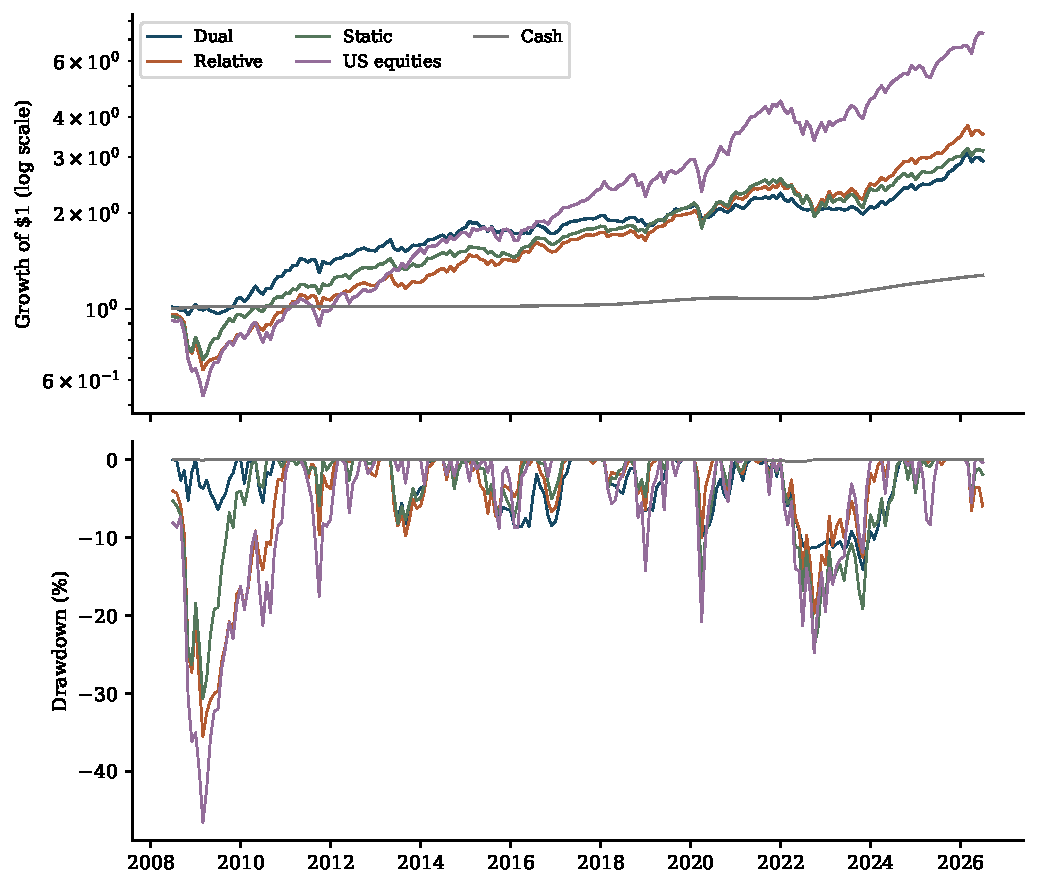
\includegraphics[width=.94\textwidth,height=.58\textheight,keepaspectratio]{../results/figures/composite.pdf}
\end{center}
All curves share June 2008--June 2026. Wealth compounds from one on a logarithmic scale. Drawdowns include initial wealth and are evaluated monthly.
\begin{center}\small\begin{tabular}{lp{10cm}}\toprule
Return month ending & Holdings at preceding month-end\\\midrule
2008-06-30 & GLD: 25\%, SHV: 75\%\\
2008-10-31 & GLD: 25\%, SHV: 75\%\\
2020-03-31 & VTI: 25\%, LQD: 25\%, VNQ: 25\%, TLT: 25\%\\
2022-06-30 & VNQ: 25\%, SHV: 75\%\\
2026-06-30 & VTI: 25\%, HYG: 25\%, REM: 25\%, GLD: 25\%\\
\bottomrule\end{tabular}\end{center}
Rows show holdings earning that month's return, selected at the preceding month-end. A sleeve contributes 25\%; SHV can combine multiple sleeves.

\newpage
\section{Module paths and diversification}
\begin{center}
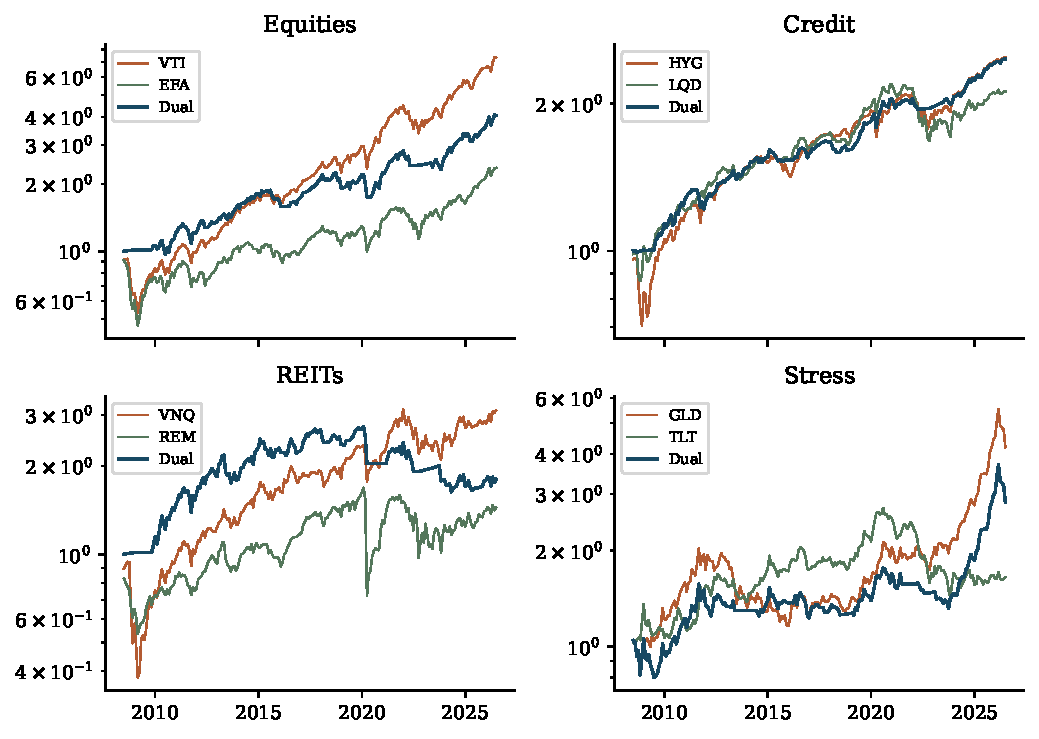
\includegraphics[width=\textwidth,height=.56\textheight,keepaspectratio]{../results/figures/modules.pdf}
\end{center}
Panels compare each module with its risky alternatives on identical dates. Logarithmic scales show proportional changes.
\begin{center}\small\begin{tabular}{lrrrr}\toprule
Module & Equities & Credit & REITs & Stress\\\midrule
Equities & 1.00000 & 0.50418 & 0.59671 & 0.01408\\
Credit & 0.50418 & 1.00000 & 0.61835 & 0.18824\\
REITs & 0.59671 & 0.61835 & 1.00000 & 0.08715\\
Stress & 0.01408 & 0.18824 & 0.08715 & 1.00000\\
\bottomrule\end{tabular}\end{center}
These are Pearson correlations of module returns. Stress has low correlations with the others. Remaining pairwise correlations are materially positive, so diversification among equity, credit and real-estate labels is incomplete.

\newpage
\section{Portfolio allocation and asset utilization}
\begin{center}
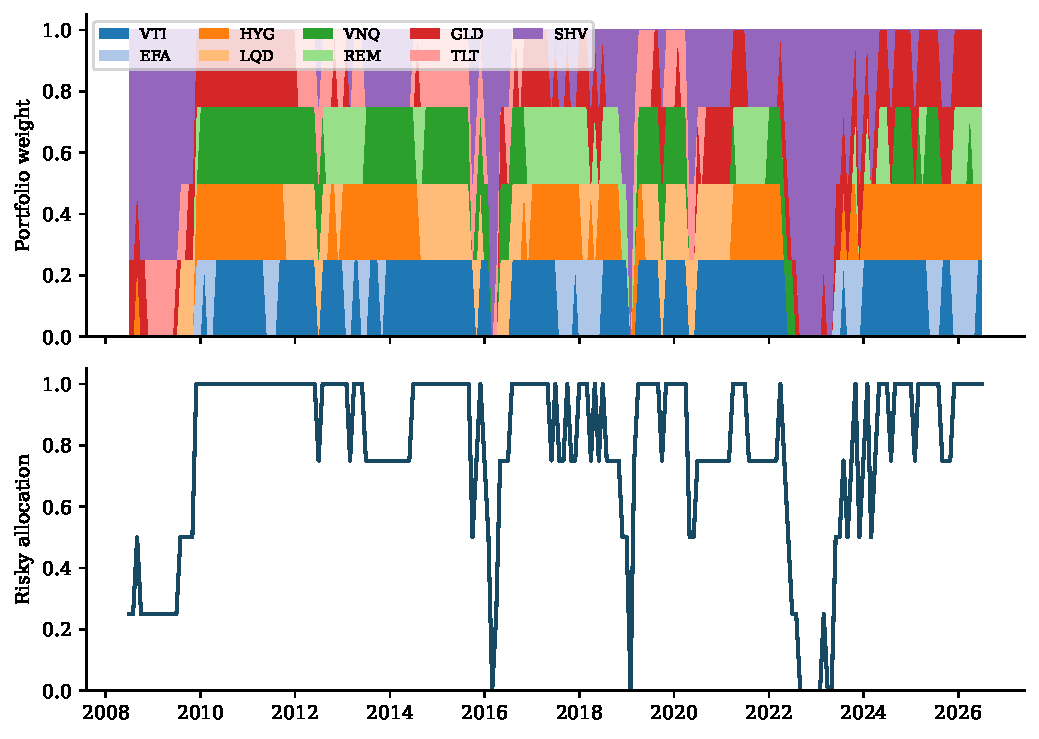
\includegraphics[width=\textwidth,height=.57\textheight,keepaspectratio]{../results/figures/allocations.pdf}
\end{center}
The area shows beginning-of-holding-month weights. The lower panel excludes SHV and measures total risky exposure.
\begin{center}\small\begin{tabular}{lrrr}\toprule
Module & First risky asset (\%) & Second risky asset (\%) & SHV (\%)\\\midrule
Equities & 64.05530 & 17.05069 & 18.89401\\
Credit & 53.91705 & 29.03226 & 17.05069\\
REITs & 46.08295 & 27.18894 & 26.72811\\
Stress & 52.53456 & 26.72811 & 20.73733\\
\bottomrule\end{tabular}\end{center}
Risky-asset order follows Section 1: VTI/EFA, HYG/LQD, VNQ/REM and GLD/TLT. Percentages sum to 100\% within a module. Utilization is selection frequency, not return contribution. Mean portfolio risky exposure is 79.14747\%.

\newpage
\section{Distributions and switching-buffer comparison}
\begin{center}
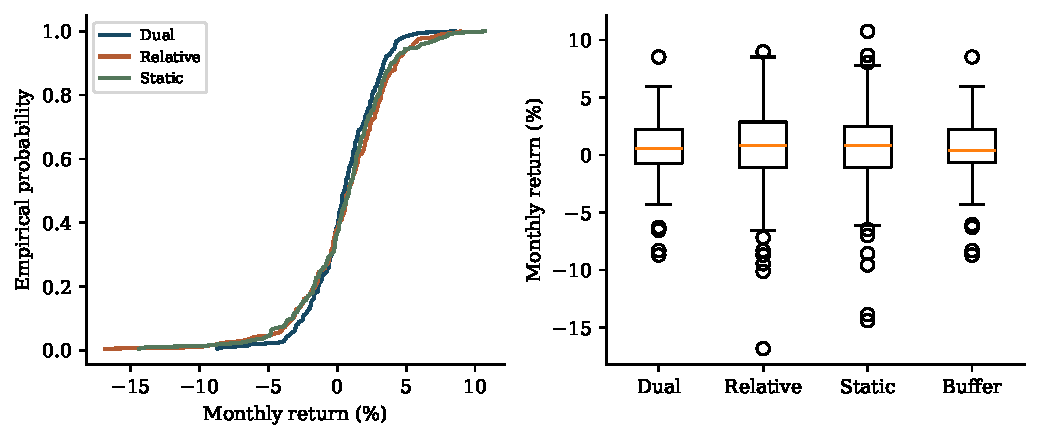
\includegraphics[width=.95\textwidth,height=.30\textheight,keepaspectratio]{../results/figures/distributions.pdf}
\end{center}
The empirical cumulative distribution includes every return. Box plots show medians, quartiles, conventional 1.5-interquartile-range whiskers and observations beyond the whiskers.
\begin{center}
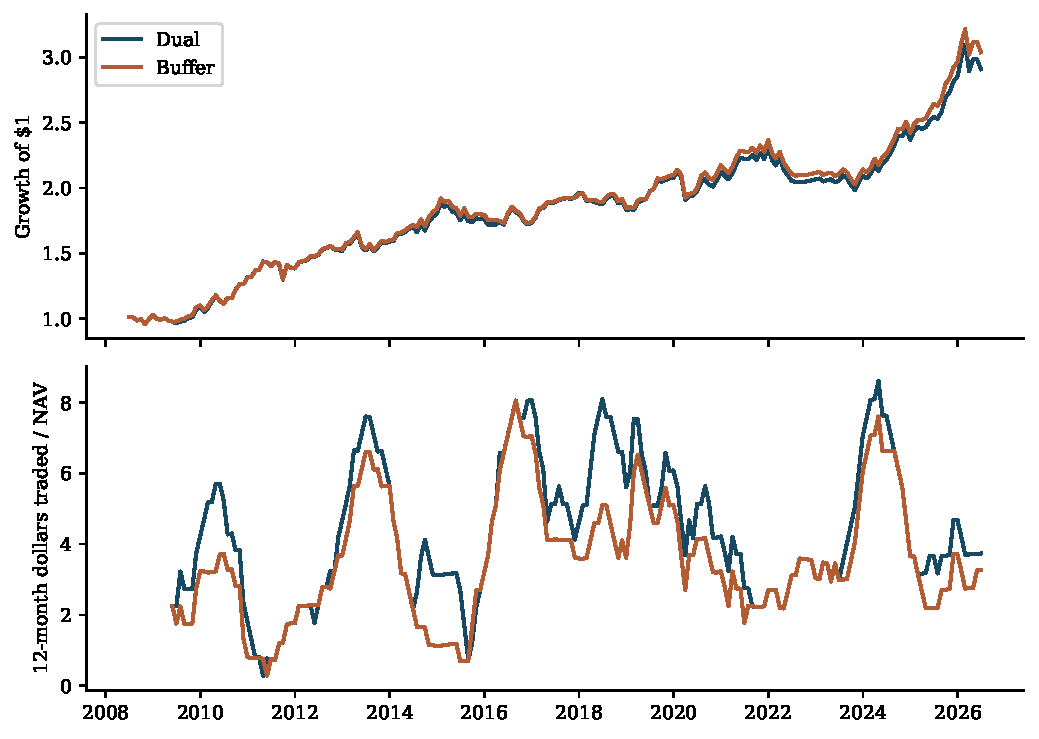
\includegraphics[width=.93\textwidth,height=.43\textheight,keepaspectratio]{../results/figures/buffer.pdf}
\end{center}
The upper panel compares gross wealth. The lower sums dollars traded over the preceding 12 months, including purchases, sales and drift rebalancing. The buffer changes relative selection only when the incumbent remains eligible under the original cash hurdle.
\end{document}
